\chapter{Background}
\label{cha:background}
\section{Literature review}
\subsection{Wearable trackers}
Consumer-based wearable fitness trackers are now readily available and can provide individuals with the ability to objectively monitor their physical activity levels. In addition, when combined with the use of smartphone and computer apps, they may assist users through a range of motivational and organisation tools to better manage their personal health \cite{trackersBenefitGeneral}.
There is plenty of research to suggest that using wearable activity trackers helps people become more physically active. A large systematic review has shown that, over several studies, there is a significant increase in daily step count, moderate and vigorous activity as a result of using wearables \cite{trackersBenefitGeneral}. In particular, people with chronic illnesses experienced decreased systolic blood pressure, waist circumference, etc \cite {Franssen2020}; monitoring such patients using wearables after hospitalizations could help detect complications and prevent rehospitalization \cite{hospi}. People of older age can also benefit greatly, showing a moderate increase in physical activity and mobility \cite{SOliveira1188}; there is an indication of good acceptability of such devices among older adults \cite {Franssen2020}. Attractiveness, gamification, readability, and feedback are what drive the health benefits such as commitment to daily physical activity \cite{NELSON2016364}. 

Wearables are not a magic bullet solution to the fitness problem. Some studies that spanned larger periods of time have observed a decrease in physical activity after an initial positive effect \cite{Finkelstein2016}, or in other words, the use of wearable devices is not directly effective at modifying habitual behaviour \cite{LI2021104487}. Many examined devices did not report sensor accuracy output validity at all, allowing for overestimation or underestimation of metrics \cite{Lee2014ActivityTA}.
\subsection{Nudging}
A nudge is “any aspect of the choice architecture that predictably alters people's behaviour without forbidding any options or significantly changing their economic incentives” \cite{nudgeDef}. An example would be providing information, implementing default choices etc. Nudges are categorised into Type 1 and Type 2. Type 1 nudge typically relies on unconscious thought and is more simple in nature, for example, rearranging the presentations of consumer items in food isles to highlight options that would have ordinarily been ignored \cite{NudgeCritical}. On the other hand, Type 2 nudge relies on conscious thought, those are more complicated and more costly, for example, long-term educational campaigns promoting exercise present the benefits of regular exercise, as well as the harmful effects of continuing to be sedentary \cite{NudgeCritical}.  

In the area of fitness, nudging has been shown to increase physical activity and reduce sedentary behaviour, for example, placing banners that encourage using the stairs displayed positive effects and an increase in stair use \cite{FORBERGER2022106922, Forberger2019}. Nudging has a lower cost of intervention than something like an educational campaign, while still being effective \cite{nudgeCost}. 

\subsection{Physical Activity}
A highly influential systematic review found "overwhelming evidence (based on millions of participants) that regular physical activity is associated with a reduced risk for all-cause mortality and several chronic medical conditions" \cite{Warburton2017Health}. Another review also supported the previous claim, as well as presenting evidence that physical activity also improves health-related quality of life, functional capacity and mood states \cite{Penedo2005Exercise}. Studies also show that those benefits can be reaped by virtually any person regardless of age, existing physical condition, etc \cite{Penedo2005Exercise, Warburton2017Health}. However, most of the benefits are gained from transitioning from sedentary to moderately active \cite{Powell2011Physical}, with some studies pointing that too much physical activity can have negative effects, such as psychological symptoms that mimic depression \cite{Paluska2000Physical} and risks of injury (for untrained individual) \cite{Melzer2004Physical}.

The Metabolic Equivalent of Task (MET) is used to express the energy cost (i.e. intensity) of physical activities as a multiple of the resting metabolic rate \cite{Jetté1990Metabolic}. An individually calculated Resting Metabolic Rate, which is calculated using a person's height, weight, age and gender should be used to calculate a more accurate MET value \cite{Byrne2005Metabolic}; this is the reason that many fitness apps ask for that information. There are tables of typical MET values for different physical activities, however, the manual calculation is inaccurate because you can complete an activity with more intensity than is typically expected \cite{Jetté1990Metabolic}; this is where wearable fitness trackers can help, automatically categorizing MET of the activity performed. One MET minute is therefore energy expanded during a minute while at rest, and it is a convenient measure for the amount of physical activity done over a time frame. For example, Walk 2 days a week at 5 METS (i.e. with moderately high intensity) for 30 minutes per session = 2 x 5 x 30 = 300 MET-minutes \cite{metMinutes}.
\subsection{Sleep}
Several papers confirm the benefits of sleep for mental health, whereby improving sleep quality had a positive effect on reducing mental health difficulties including depression and anxiety \cite{sleep1, sleep2, sleep3}. Disturbances, such as irregular sleep starts can also impact the physical body, weakening the immune system \cite{sleep4} and changing metabolic regulation \cite{sleep2}.

Sleep is made of many stages, but 3 large groups are: light sleep, deep sleep and rapid-eye-movement (REM) sleep; These stages have close ties with heart-rate variability during those stages \cite{sleepDef}. During deep sleep, muscles relax, which promotes their recovery \cite{Jung2010Energy}. REM sleep is essential for normal body physiology, ensuring recovery from sleep and return to consciousness \cite{VERTES1986371}. Wearable devices primarily use heart rate and its variability to determine the sleep stages throughout the night, although other metrics such as skin conductance and temperature may be used as well \cite{Zambotti2019Wearable}. The state-of-the-art method for derivation of sleep stages and sleep quality is using deep learning \cite{Sathyanarayana2016Sleep}.

\section{Similar Systems}
\label{section:similarSystems}
\subsection{Google Fit}
Google Fit is an open ecosystem. It lets developers upload health and wellness data to a central repository where users can access their data from different devices and apps in one location \cite{googleFit}. All types of health data are supported except for something specialised like an ECG. Its defining good qualities are a very clean UI, completely free with no ads and a relatively cross-platform app, with iOS and Android supported, but no web version.  Google Fit by itself offers very limited functionality, such as the dashboard of aggregated data - it is a platform. Other apps can connect to that aggregated data and use it for useful purposes, but they can still use it unethically. Google Fit is still a closed-source system, which does not make any money, so it is not clear how Google covers those expenses. Google was involved in many legal cases with EU courts for anti-trust \cite{googleAntiTrust} and data protection violations \cite{googleDataProtect, googleDataProtect2}.
\subsection{Apple Health \& Apple Fitness+}
Apple Health is essentially the same as Google Fit, with the basic version also just providing a simple dashboard. But, unlike Google, it offers a premium service - Apple Fitness+ with a cost of 9.99£, which offers health reports, trends and exercise plans. It is well integrated into the Apple product ecosystem. The biggest downside is that it is only available on iOS devices as an app. Apple Health is a good option for users with iOS devices, as the company has a generally good reputation with data privacy, but there were small cases of GDPR violations \cite{CNILApple} and major cases of anti-trust \cite{appleAntiTrust}.
\subsection{MyFitnessPal}
MyFitnessPal is an app described with: "Build healthy habits with the all-in-one food, exercise, and calorie tracker" \cite{fitnesspal}. Its free version contains the same basic functionality, such as syncing data and showing it on a dashboard. Anything more useful like reports, guided exercise routines, etc is behind a premium costing 15.99£ per month. One very impressive feature is the meal scan, where meals are added by pointing a camera at them. It has a negative reputation, experiencing a major data breach involving 150 million users \cite{masuch2021fitness, myFitnessPalDataBreach}, transferring data to the US \cite{myfitnesspalTransferring} where data protection laws are more lenient and pay-walling previously free features \cite{myfitnesspalPaywall}.

\section{Devices Used}
\subsection{Withings}
\label{section:WithingsWatch}
Withings ScanWatch was used for the project - \cite{withingsStorePage}. It can record activity seconds, steps, ECG (electrocardiogram - waveform of heart's electrical activity), SPO2 (blood oxygenation) and more. ScanWatch integrates a different device called Scan Monitor, which has CE medical certification in Europe and FDA clearance in the United States \cite{withingsStorePage}.  Scan Monitor has the following accuracy metrics published \cite{scanMonitor}:
\begin{itemize}
    \item ECG recording: IEC 60601-2-47 (Requirements for the Basic Safety and Essential Performance of Ambulatory Electrocardiographic Systems.) beat-to-beat detection with F1-score of at least 99.19\%.
    \item AFib: 98.16\% sensitivity in classifying AFib (irregular heartbeat).
    \item Sinus Rhythm: 97.20\% specificity in classifying sinus rhythm.
\end{itemize}
SPO2 accuracy is provided by this statement: "The measure of SpO2 in the range 70-100\% has been clinically validated on healthy adult volunteers, at rest against a laboratory co-oximeter" \cite{scanMonitor}.
Other metrics do not seem to have any accuracy declarations. Assuming that those are derived, rather than measured directly. For example, for breathing disturbances, the website notes: "Our exclusive algorithm, developed with experts, computes the data from SpO2, heart rate, motion and breathing rate to measure breathing disturbances, an indicator of sleep apnea". During the app set-up, only when enabling ECG, AFib and SPO2 do you have to accept the accuracy document. This implies that only those metrics are certified medical-grade, while others are not.

The watch has been used in peer-reviewed studies:
\begin{itemize}
    \item Examining if remote monitoring (using the watch + other) improved outcomes of patients undergoing hip and knee arthroplasty: statistically significant reduction in rehospitalization rate in the intervention arm \cite{withingsHospitalization}
    \item Examine large cohorts for the presence of Nocturia (waking up to urinate at night) in natural settings using the watch: watch made it possible to discover an association \cite{withingsNocturia}.
\end{itemize}


\subsection{Oura}
\label{section:OuraRing}
Oura Generation 2 ring was used for the project - \cite{ouraStorePage}. Oura does not call the device "medical-grade" unlike Withings, since it carries a need for medical certification. Instead, they call it "research-grade". Oura publishes its sleep tracking accuracy metrics, showing 79\% agreement with gold-standard polysomnography (PSG) for 4-stage sleep classification (wake, light, deep, and rapid eye movement (REM) sleep) \cite{OuraSleepAcc}. Also, sleep heart rate and heart rate variability have high degrees of accuracy \cite{ouraHeartAcc}; the study also notes the ring's memory limitation, as two days old data is lost if the user doesn't open the app. 

Oura was also used in peer-reviewed studies:
\begin{itemize}
    \item Used Oura ring to measure the peripheral temperature of subjects who then reported COVID-19: showed wearable sensors (Oura ring) can detect illness in the absence of symptoms \cite{smarr2020feasibility}.
    \item Used Oura ring to measure distal body temperature to predict pregnancy earlier than pregnancy test: able to generate hypothetical alert a median of 9 ± 3.9 days before the date individuals received a positive pregnancy test \cite{ouraPregnancy}.
\end{itemize}
\section{Software Requirements}
There 3 different types of requirements relevant to the domain of software: user requirements describing goals that a specific class of user must be able to perform, functional requirements describing what developers must implement to enable users to accomplish tasks (user requirements), business requirements describing the high-level business objective of the organization that builds the system and optionally non-functional requirements, describing more qualitative features the system should have \cite{wiegers2013software}. Compiling these requirements helps us understand features more deeply and negotiate project scope \cite{Damian2006An}. The only business requirement for this project is minimising cost, because it is open-source it won't bring any profit to creators.

User requirements can be understood by a non-technical person. They can be represented using user stories. User story represents requirements using a simple textual template: "As a [role] I can [capability], so that [receive benefit]" \cite{userStories}. Acceptance criteria may also be attached to a user story, containing details under which testable conditions the story can be considered completed \cite{Kannan2019User}. One of the popular templates for an acceptance criteria is: " Given [conditions], When [action taken], Then [outcome of action taken]". 

Functional requirements are more technical and are intended to be used as a description of a system that engineers need to implement \cite{wiegers2013software}. Although purely textual representations exist, more detailed representations that utilize diagrams are preferred. (System) Use case diagram is a UML diagram used to specify functionality offered by the system \cite{malan2001functional}. Requirements with lots of conditionals can be represented as a flow chart, or if the requirement is simple, it could be represented as a sentence in the style of a user story. 

To give a brief introduction to a system use case diagrams: \ref{fig:useCase}
\begin{itemize}
    \item Extend: base use case is complete by itself. Extending use case is optional.
    \item Include: base case is incomplete, included use case is a required.
    \item Implements: use case is abstract.
\end{itemize}
\begin{figure}
    
    \centering
    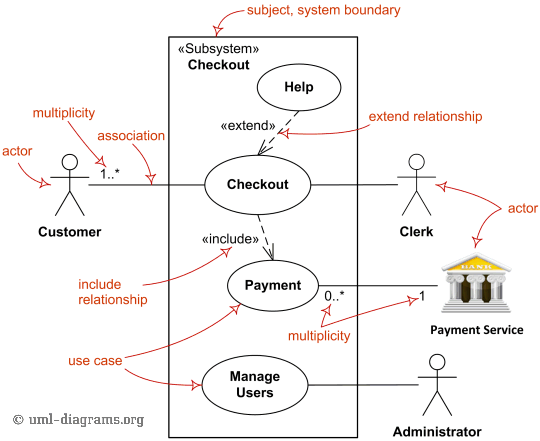
\includegraphics[width=0.9\textwidth,keepaspectratio]{../images/use-case-diagram-elements.png}
    \caption{System use case diagram}
    \label{fig:useCase}
\end{figure}

\section{Cloud}
Cloud computing is a model for enabling convenient, on-demand network access to a shared pool of configurable computing
resources (e.g., networks, servers, storage, applications, and services) that can be rapidly provisioned and released with minimal management effort or service provider interaction \cite {cloudDef}.
Using cloud for the software service infrastructure has the benefit of off-loading complexity to cloud providers instead of handling it yourself. In comparison with traditional in-house infrastructure, cloud is superior in terms of cost, as there is no upfront cost and it generally being cheaper through economies of scale, as well as and reliability, as maintenance and contingency planning are handled by the best specialists in that area \cite{armbrust2009above, hajjat2010cloudward}.  
\subsection{Serverless \& Microservices}
Serverless computing differs from traditional cloud computing, as the infrastructure on which services are running is hidden from customers so that they only need to worry about desired application functionality rather than configuration and management of low-level resources; Also provides pay-as-you-go model and auto-scaling per demand \cite{serverless1}.  It is mainly used in Event-Driven systems because successful application of serverless requires well-defined: event, trigger and action \cite{MALAWSKI2020502, serverless2}. 

Monolithic architecture means that an application runs as a single process in the application server's environment, there maybe multiple servers, but they are just replicas running the same application. It's main benefit is simplicity, being easier to develop, test and deploy \cite{monolith}.

Microservices architecture on the other hand partitions the functionality of the application into a set of small services and making them communicate with each other through light weight mechanisms (e.g., RESTful API) \cite{fowler2014eb}. The benefits are scalability, agility, availability and security; for example, when a bug crashes the service in a monolith, the whole service is shut down, whereas in microservices, only the service with the bug is shut down, and that service may not be fully needed for operations; there could be redirects to another slightly worse service, so the service as a whole can still function. However there are also negatives, most notably performance and latency, as communication is usually via network \cite{Li2021Understanding}, therefore slower than monolithic intra-process communication. This approach became popular after Netflix pioneered it and migrated their service to use microservices, after experiencing a catastrophic service outage \cite{monolith}.
% TODO add that it is microservice, adds fault tolerance.
\subsection{Cloud Providers}
There are 3 major providers in this space: AWS, Azure and GCP. They fall into the public cloud category, similar to utility services like electricity, they are available for use to anyone, be it an individual developer or a company. Providers outline their legal promises in the document called Service Level Agreement (SLA) \cite{cloudSLA}.

AWS was chosen for this project for the following reasons:
\begin{itemize}
    \item{AWS has the best security system \cite{Narula2015Cloud}, mainly due to IAM, tightly controlling what each entity is allowed to access in the infrastructure. As well as being the most trusted provider, never facing major outages or security breaches (where the fault was on AWS itself).}
    \item{if used under similar conditions, AWS has among the best quantitative performance metrics, such as availability, latency etc. \cite{CloudMetrics}.  }
    \item {I have a lot of experience working with AWS, so I can get started on the project faster.}
\end{itemize}
\subsection{AWS Components}
\begin{itemize}
    \item Lambda: Serverless function offering which allows deployment of microservices without the need of managing servers with pay only for what you use pricing structure \cite{LambdaCostSave}, also referred to as Function-as-a-Service model \cite{MALAWSKI2020502}. Function is executed in response to an event, such as a direct HTTP call.  Allows saving up to 77.08\% compared to traditional monolithic server \cite{LambdaCostSave}.
    \item DynamoDB: a fully managed NoSQL database that provides predictable and super-fast performance with unified scalability. Defining Characteristics: Eventually consistent, AP in CAP classification and key-based access focus \cite{DynamoDB}. Tables are schemaless except for the Primary key, which has to be unique among the rows; it may consist of a Partition key or composite of Partition key + Sort key, with partition determining internal physical storage partition and items being sorted in order via sort key attribute \cite{awsDynamoWebsite}. 
    \item SNS: Amazon Simple Notification Service (Amazon SNS) is a managed service that provides message delivery from publishers to subscribers (also known as producers and consumers). Publishers communicate asynchronously with subscribers by sending messages to a topic, which is a logical access point and communication channel. Clients can subscribe to the SNS topic and receive published messages using a supported endpoint type \cite{sns}. 
    \item Amplify: AWS Amplify is a complete solution that lets frontend web and mobile developers easily build, connect, and host full-stack applications on AWS \cite{amplify}. Although it has a lot of services, only Amplify Hosting will be used. It provides a git-based workflow for continuous deployment and subsequent hosting: performing typical front-end server functionalities: file compression, caching, etc.
\end{itemize}
The following diagram gives a visual representation of each above-mentioned component: \ref{fig:awsComponents}.
\begin{figure}
    
    \centering
    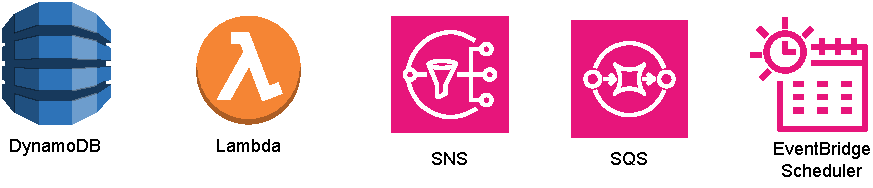
\includegraphics[width=0.95\textwidth,keepaspectratio]{../images/AWS_components.pdf}
    \caption{AWS diagram component labelling}
    \label{fig:awsComponents}
\end{figure}
\subsection{Security}
Software Security is important, especially in the context of this project, as it deals with sensitive health data. Generic web security recommendations should apply to this project, such as encrypting the data in transit. However, deploying the application on the cloud presents new security issues \cite{Zissis2012Addressing}, requiring stricter planning and evaluation.

Voluntary Application Server Identification (VAPID) is an authentication method for WebPush (push protocol for web). It uses public and private keys to make sure that only the intended server can send push notifications to a client \cite{vapid}.

Cross Site Scripting (XSS): a JavaScript code injection attack which happens when untrusted user input is used in a web application \cite{gupta2017cross}. 

Clickjacking: An exploit when the website is embedded via iframe on the attacker's website and original UI elements are masked behind fake ones \cite{clickjacking}.

Content-security policy (CSP): Mitigates XSS by defining from which origins (urls) files are considered valid, with all other files rejected \cite{csp}.

Strict Transport Security: Force all communication to happen through HTTPS, else don't allow the communication to happen \cite{hsts}. 
\section{LLMs}
"A large language model is the language model with massive
parameters that undergoes pretraining tasks (e.g., masked
language modelling and autoregressive prediction) to understand and process human language, by modeling the
contextualized text semantics and probabilities from large
amounts of text data" \cite{Yao2023ASO}.
Unlike other machine learning models, the main way to improve response quality is to improve the prompt \cite{Liu2021PretrainPA}; "Prompt Engineering" is the technique for doing that, maximizing the utility of LLMs in various tasks \cite{zhou2023large}. The following techniques were discovered:
\begin{itemize}
   \item Retrieval Augmented Generation (RAG): RAG is a functionality that allows LLMs to access relevant external knowledge and use it for response generation. It is usually more prioritised than the ordinary context, significantly reducing the chances of hallucinations and improving output quality \cite{gao2024retrievalaugmented}.
   \item Few-Shot prompting:  providing hand-crafted examples of good replies to an input, has shown to provide better model performance \cite{brown2020language, min2022rethinking}. When 1 pair is provided it is called 1-shot prompt, 5 - 5-shot, etc. 
   \item Chain of Thought (CoT) prompting: when utilising few-shot prompting, providing intermediate reasoning steps in the example reply improves performance as well as enables complex reasoning capabilities \cite{wei2023chainofthought}. There is a zero-shot version i.e. prompt without examples. Providing a "magic" phrase at the end of the prompt: "Let's think step by step" improves performance over the default prompt and rivals few-shot prompts \cite{kojima2023large}.
   \item Details, Persona: According to OpenAI \cite{openAI}, including more details and asking the model to assume a persona, like a personal trainer, can improve reply relevancy. 
\end{itemize}
 In 2022, OpenAI made GPT3 available to the public, a product that surpassed Google in daily web page visits. It revolutionized AI, in a way that a lay person could use it with some decent efficiency. The vital factor is its ability to effectively use a context window, a collection of prior information (such as prior messages sent in a chat) that is used to influence the next output. GPT4 is the latest version, it has better performance but is also pricier. The workflow of using GPT4 API: Explicitly attach context messages with a prompt. The complexity of managing contexts was upon your system that uses the OpenAI API. This recently changed with Assistants API. This feature allows creation of assistants, which can have threads that correspond to continuous chat with a user. The key factor is that the complexity of maintaining context is handled by OpenAI. Also, it features OpenAI's own Retrieval Assisted Generation (RAG) solution named Knowledge Retrieval. 

 One limitation of Large Language Model (LLM) content generation is hallucination, or false assertions in the generated text \cite{ji2023survey}.

\section{UI}
\label{section:goldenRules}
Ben Shneiderman's eight golden rules of UI design are widely regarded as a good framework for designing and evaluating UIs. It comprises 8 simple rules that a good UI should follow \cite{goldenRulesUI}: \begin{itemize}
    \item Strive for consistency: page contents should mostly be consistent, such as fonts, colours etc. 
    \item Seek universal usability: everyone can use the product
    \item Offer informative feedback: user's actions should have an observable impact.
    \item Design dialogues to yield closure: confirm that something failed or succeeded, never leave users not knowing what is going on.
    \item Prevent errors: when possible, restrict actions available so that the user can't make obvious errors.
    \item Permit easy reversal of actions: actions should be reversible.
    \item Keep users in control: make it easy for users to accomplish their desired results.
    \item Reduce short-term memory load: don't show too much information at once.
\end{itemize}

\section{Data analysis \& Statistical Testing}
\subsection{Bland-Altman Plot}
Bland-Altman plot is a general method for visualizing differences between measurements of two methods. The Bland-Altman (BA) graph consists of a scatter plot in which the difference between two measures (Test \#1 - Test \#2) is constructed on the vertical axis, while the mean of the two measures ([Test \#1 + Test \#2]/2) is depicted on the horizontal axis \cite{kaur2017bland}. Limits of agreement may also be drawn. They signify boundaries of difference, beyond which points would be more than x standard deviations away from the mean difference; 1.96 SD is commonly used \cite{myles2007using}.  In particular, it is used extensively in medical research, when there is a need to determine if two methods can be used interchangeably \cite{myles2007using}.
\subsection{Outlier detection - Z-score}
Z-score also known as Standard score, is the number of standard deviations by which a data point is above or below the mean of the population. Ideally, it requires knowing the population mean and standard deviation (SD), however, for practical reasons those are estimated with the sample's stats; It is calculated by: $z=\frac{x-\hat{x}}{SD}$ \cite{zscoreBook}. It can be used for outlier detection, such as data points more than 2 SDs away are considered outliers, i.e. data points with $\text{abs}(z) >= 2$ are outliers.
\subsection{Hypothesis testing}
Student's t-test is a statistical testing method to test a hypothesis of whether the population means of 2 groups are different with a certain confidence. It is often the preferred choice over Z-test, as it does not require knowing the population's mean and SD; instead, those are estimated from the sample and corrected with degrees of freedom according to the sample size. Independent t-test assumes equal variance between 2 groups, whereas the Paired version does not assume equal variance. Paired version should be used when two groups depend on one another \cite{LIVINGSTON200458}, such as when measuring the temperature of the same person with different thermometers.

Two one-sided tests (TOST) also allow testing whether the population means of 2 groups are different, however, we can also define bounds on what is considered a worthwhile difference - these are called equivalence bounds; Basically, we can test whether the difference between groups is significantly larger than some defined tolerance bounds, instead of just testing whether there is any difference \cite{tost}.
% On 4th March 2024, Shortly after finishing the project implementation, Anthropic announced Claude 3 Sonnet. It's benchmark scores are similar or better than gpt-4-1106-preview, it has bigger context window but costs 333\% less. This makes the reasoning behind the choice of gpt-4-1106-preview not valid at the moment of writing the report, however it was valid at the time of planning for AI functionality at the time of Dec 2023. 